\documentclass[conference]{IEEEtran}
\usepackage{cite}
\usepackage{amsmath}
\usepackage{textcomp}
\usepackage{xcolor}
\usepackage{booktabs}
\usepackage{url}
\usepackage{tikz}
\usetikzlibrary{shapes.geometric, arrows.meta, positioning, calc}
\usepackage[hidelinks]{hyperref}

\begin{document}

\title{synth-attest: An Open, Vendor-Neutral Verifiable-Identity and\\
Tamper-Evident Audit Layer for DNA-Synthesis Order Compliance}

\author{\IEEEauthorblockN{Pavan Kumar Dubasi}
\IEEEauthorblockA{Independent\\
pavankumar.dubasi2019@gmail.com}}

\maketitle

\begin{abstract}
DNA-synthesis screening answers whether a sequence is dangerous, but not who ordered it,
whether they are a verified researcher, or whether a trustworthy record of the decision exists.
As regulation (the proposed US Biosecurity Modernization and Innovation Act, the US OSTP
framework, UK DSIT guidance, and the proposed EU Biotech Act) converges on mandating customer
identity verification and recordkeeping, no shared, vendor-neutral tooling exists; commercial
entrants use centralized, per-provider Know-Your-Customer (KYC) workflows. We present
synth-attest, an open-source layer that sits on top of (and never replaces) sequence screening,
adding three capabilities built on W3C standards: a portable researcher-identity credential, a
provider-issued revocable exemption credential, and a privacy-preserving, tamper-evident
order-audit record. The design is vendor-neutral by construction: the core has zero proprietary
dependencies and runs on a dependency-free reference engine, with any W3C Verifiable Credential
backend pluggable behind a stable interface. We report a working prototype (592 lines of core
Python, 33 tests) validated in continuous integration on Python 3.11 and 3.12 in two
configurations: a no-proprietary-dependency core (23 passed, 10 backend tests skipped) and an
optional backend validated source-blind against its published package (33 passed). We state the
threat model honestly, scoping the contribution to fraud, attribution, and deterrence at the
acquisition node.
\end{abstract}

\begin{IEEEkeywords}
biosecurity, DNA synthesis, verifiable credentials, decentralized identifiers, audit trails,
know-your-customer, compliance
\end{IEEEkeywords}

\section{Introduction}
Advances in machine learning lower the barrier to designing biological sequences of concern,
making the nucleic-acid synthesis-order step one of the few remaining physical chokepoints for
governance. Sequence-screening systems such as SecureDNA~\cite{securedna} and the IBBIS Common
Mechanism~\cite{ibbis} assess whether an ordered sequence matches a hazard, but they do not
establish \textit{who} is ordering, whether that customer is a verified and legitimate
researcher, or whether the order decision leaves a tamper-evident, independently verifiable
record. Recent and proposed regulation, including the US Biosecurity Modernization and
Innovation Act of 2026~\cite{s3741}, the US OSTP nucleic-acid-synthesis framework, UK DSIT
screening guidance~\cite{dsit}, and the proposed EU Biotech Act, pushes providers toward
customer identity verification and recordkeeping. No shared, portable tooling exists to meet
these obligations; commercial entrants address them with closed, per-provider KYC workflows.

We present \textbf{synth-attest}, an open, vendor-neutral layer that adds the missing identity
and audit capabilities on top of existing screening. It is deliberately scoped: it does not
screen sequences and never handles sequence data.

\section{Threat Model and Honest Scope}
We map the engineered-pandemic kill chain as: capability uplift, acquire materials, synthesize,
weaponize, release. synth-attest intervenes at a single node, \textit{acquire materials}, and
only for actors routing through compliant providers. It addresses three failure modes there:
identity fraud (spoofed or unverified customers), weak attribution (no portable record of who
ordered what), and low deterrence. It explicitly does \textit{not} address capability uplift,
benchtop or non-compliant synthesis, weaponization, or a genuinely credentialed malicious
insider; identity proves identity, not intent. Any claim that the layer ``prevents engineered
pandemics'' is unsupported and avoided.

\begin{figure}[t]
\centering
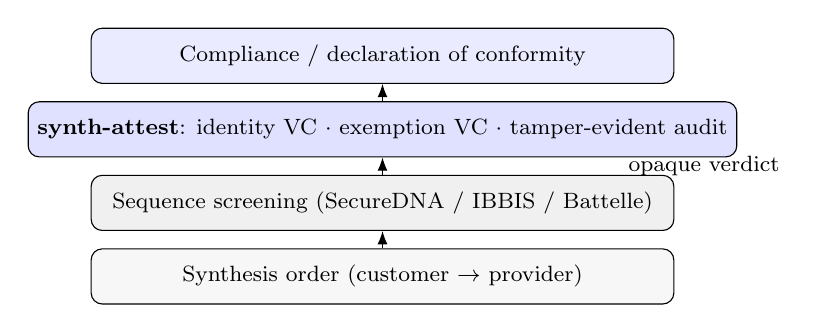
\begin{tikzpicture}[font=\footnotesize, node distance=2.2mm,
  layer/.style={draw, rounded corners, minimum width=7.4cm, minimum height=7mm, align=center}]
\node[layer, fill=blue!8] (compliance) {Compliance / declaration of conformity};
\node[layer, fill=blue!12, below=of compliance] (synth) {\textbf{synth-attest}: identity VC $\cdot$ exemption VC $\cdot$ tamper-evident audit};
\node[layer, fill=gray!12, below=of synth] (screen) {Sequence screening (SecureDNA / IBBIS / Battelle)};
\node[layer, fill=gray!6, below=of screen] (order) {Synthesis order (customer $\rightarrow$ provider)};
\draw[-{Latex}] (order) -- (screen);
\draw[-{Latex}] (screen) -- (synth) node[midway, right, xshift=3.0cm] {opaque verdict};
\draw[-{Latex}] (synth) -- (compliance);
\end{tikzpicture}
\caption{Layered architecture. synth-attest adds an identity and audit layer above sequence
screening, which it never replaces. Only an opaque verdict (cleared / flagged / tier-review)
crosses the boundary; no sequence data enters the layer.}
\label{fig:arch}
\end{figure}

\section{Design}
synth-attest provides three artifacts and one privacy property (Fig.~\ref{fig:arch}).

\subsection{Portable researcher-identity credential}
A W3C Verifiable Credential~\cite{w3cvc} bound to a Decentralized Identifier~\cite{w3cdid}
asserts a verified researcher and institutional affiliation only. It is explicitly not a
clearance, and carries no risk-tiering field. Portability lets a researcher avoid re-onboarding
at every provider, addressing the documented gap that customer screening is currently
re-performed per provider and rarely shared.

\subsection{Provider-issued exemption credential}
Following existing exemption-certification practice, an exemption credential is issued by the
provider (which retains regulatory liability) to authorize a sequence \textit{class}, never a
sequence. It is time-bound and revocable. This separates the portable identity (about the
person) from the order-specific authorization (the provider's local decision), correcting a
common conflation between credentialing a person and clearing an order.

\subsection{Privacy-preserving tamper-evident audit}
Each order decision produces an append-only, signed record held by the provider. Only a salted
SHA-256 commitment over (salt, order id, verdict, customer DID) is anchored, and commitments are
anchored in fixed-size batches of $B=16$, padded with indistinguishable random fillers and
sorted, so that order volume, timing, and the screening verdict are not recoverable from what is
anchored. A customer-facing receipt never contains the verdict, preventing the audit channel
from becoming a screening-evasion oracle.

\subsection{Infohazard guard}
No sequence-like data may enter the layer. A guard rejects any payload containing a
nucleotide-alphabet (\texttt{[ACGTU]}) run of length $\geq 20$, erring toward false positives,
the safe direction for an infohazard boundary.

\begin{figure}[t]
\centering
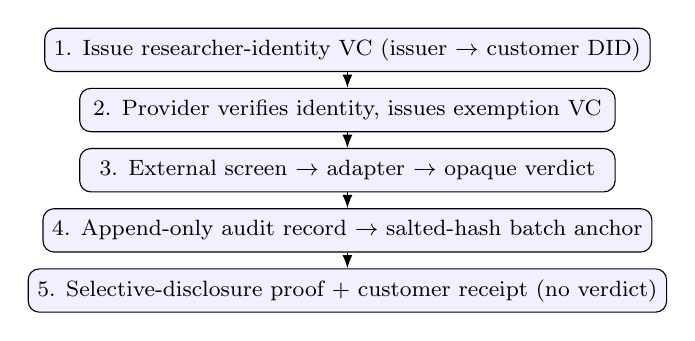
\begin{tikzpicture}[font=\footnotesize, >={Latex},
  flowstep/.style={draw, rounded corners, fill=blue!6, minimum width=6.8cm, minimum height=5.5mm, align=center}]
\node[flowstep] (s1) {1. Issue researcher-identity VC (issuer $\rightarrow$ customer DID)};
\node[flowstep, below=2mm of s1] (s2) {2. Provider verifies identity, issues exemption VC};
\node[flowstep, below=2mm of s2] (s3) {3. External screen $\rightarrow$ adapter $\rightarrow$ opaque verdict};
\node[flowstep, below=2mm of s3] (s4) {4. Append-only audit record $\rightarrow$ salted-hash batch anchor};
\node[flowstep, below=2mm of s4] (s5) {5. Selective-disclosure proof + customer receipt (no verdict)};
\draw[->] (s1)--(s2); \draw[->] (s2)--(s3); \draw[->] (s3)--(s4); \draw[->] (s4)--(s5);
\end{tikzpicture}
\caption{End-to-end order flow, implemented as the project demo and runnable on both engines.}
\label{fig:flow}
\end{figure}

\section{Vendor Neutrality}
The core has zero proprietary dependencies. A dependency-free reference engine
(\texttt{StubEngine}) implements the full contract (issue, verify, detect tampering, revoke,
selectively disclose), so the entire flow runs with only the Python standard library. A
swappable \texttt{CredentialEngine} interface allows any conformant W3C VC/DID backend; an
optional adapter (\texttt{AttestixEngine}) is provided but not required, and auto-detects the
backend's service or functional surface. Continuous integration enforces independence: one job
installs the core, \textit{asserts the optional backend is absent}, and runs the suite; a second
installs the optional backend and validates it source-blind against the published package.

\section{Implementation and Validation}
The prototype is 592 lines of core Python across five modules (engine, schemas, audit, adapters,
custody), plus reference adapters that map SecureDNA-shaped and IBBIS-Common-Mechanism-shaped
screening results to the three opaque verdicts, and a custodial registry so researchers need not
operate a key wallet (a provider or neutral registry custodies the credential, keyed by a
salted hash of an identifier). Every credential and audit field is traced to a named regulatory
obligation, each marked verified or unverified, and a test fails if any schema field lacks a
mapping row. Table~\ref{tab:artifacts} summarizes the artifacts; Table~\ref{tab:results} reports
validation. The suite is 33 tests; in the no-proprietary-dependency configuration 23 pass and
the 10 backend-specific tests skip, and with the optional backend active (validated source-blind
against the published package) all 33 pass. Both configurations are green in CI on Python 3.11
and 3.12.

\begin{table}[t]
\caption{Artifacts and their key properties}
\label{tab:artifacts}
\centering
\renewcommand{\arraystretch}{1.2}
\begin{tabular}{@{}lll@{}}
\toprule
\textbf{Artifact} & \textbf{Issuer} & \textbf{Key property} \\
\midrule
Researcher identity VC & registry & portable; identity only, no tier \\
Exemption VC & provider & sequence-\textit{class}, time-bound, revocable \\
Order audit record & provider & salted SHA-256, batch $B{=}16$ anchor \\
Disclosure proof & holder & selective; reveals chosen fields only \\
\bottomrule
\end{tabular}
\end{table}

\begin{table}[t]
\caption{Validation results (continuous integration)}
\label{tab:results}
\centering
\renewcommand{\arraystretch}{1.2}
\begin{tabular}{@{}lcc@{}}
\toprule
\textbf{Configuration} & \textbf{Passed} & \textbf{Skipped} \\
\midrule
Core only (no proprietary dependency) & 23 & 10 \\
Optional backend (source-blind, published) & 33 & 0 \\
\midrule
\multicolumn{3}{@{}l}{Python 3.11 and 3.12; 33 tests collected; 592 LOC core.} \\
\bottomrule
\end{tabular}
\end{table}

Three properties are demonstrated by dedicated tests rather than asserted: (i) tampering with any
credential field causes verification to fail; (ii) a revoked credential fails verification and
cannot be presented; and (iii) the anchored batch root has fixed width and does not reveal the
number of real orders in the batch, so order volume is not recoverable from what is anchored.

\section{Related Work and Positioning}
Sequence-screening systems~\cite{securedna,ibbis} are complementary, not competing; synth-attest
consumes their verdicts as opaque tokens. Commercial KYC entrants for synthesis providers use
centralized identity verification and per-provider recordkeeping. The distinguishing properties
of synth-attest are portable W3C credentials, cross-provider tamper-evident audit, and an open,
vendor-neutral implementation, none of which the centralized approaches provide.

\section{Limitations and Future Work}
The reported results are functional and integration tests of a prototype, not an empirical study
of deployed effectiveness. The exemption and audit models are validated against published
descriptions of real screening practice but not yet against a live provider integration. A
credential-tiering field is deliberately omitted pending confirmation that any real framework
tiers researcher clearance rather than data sensitivity. An issuer trust-root design (accrediting
identity issuers without recreating a centralized authority) is the principal open architectural
question. Throughput and anchor-cost at realistic order volumes, and a live screening
integration, are the next validation steps.

\section{Conclusion}
synth-attest supplies the identity and audit layer that sequence screening leaves open, as an
honest, narrowly scoped, and vendor-neutral open-source contribution to nucleic-acid synthesis
governance.

\appendices
\section{Reproducibility of reported figures}
All numeric claims are mechanically checkable from the public repository at the cited commit:
592 LOC (\texttt{wc -l src/synth\_attest/*.py}); 33 tests collected (\texttt{pytest --co});
23 passed / 10 skipped core and 33 passed with the optional backend (\texttt{pytest});
batch size $B{=}16$ and the SHA-256 commitment (\texttt{src/synth\_attest/audit.py}); the
length-20 \texttt{[ACGTU]} guard (\texttt{src/synth\_attest/schemas.py}); optional backend
version pinned in \texttt{pyproject.toml}. The two CI configurations are defined in
\texttt{.github/workflows/ci.yml}.

\begin{thebibliography}{00}
\bibitem{securedna} SecureDNA Foundation, ``Verifiably and privately screening global DNA
synthesis,'' 2024. \url{https://securedna.org/}
\bibitem{ibbis} International Biosecurity and Biosafety Initiative for Science, ``The Common
Mechanism for DNA Synthesis Screening.'' \url{https://ibbis.bio/common-mechanism/}
\bibitem{s3741} US Senate, ``Biosecurity Modernization and Innovation Act,'' S.3741, 119th
Congress, 2026.
\bibitem{dsit} UK Department for Science, Innovation and Technology, ``Screening guidance on
synthetic nucleic acids for users and providers,'' 2024.
\bibitem{w3cvc} W3C, ``Verifiable Credentials Data Model,'' W3C Recommendation.
\bibitem{w3cdid} W3C, ``Decentralized Identifiers (DIDs) v1.0,'' W3C Recommendation, 2022.
\end{thebibliography}

\end{document}
